% Chapter 6: Discretization Invariance and Continuum Limits
% Part I of the book.

\chapter{Discretization Invariance and Continuum Limits}
\label{ch:part1-discretization-invariance-and-continuum-li}
\label{sec:discretization}
% -----------------------------------------------------------------------------

Every number a neural operator returns is computed on a grid, yet the
architecture itself is defined on function spaces.
Reconciling those two facts is the task of this chapter. Discretization
invariance\index{discretization invariance} is the property most often advertised for neural operators and the
most often overstated: it is casually read as meaning that a trained network is
accurate at any resolution, that mesh refinement costs nothing, and that the
implemented network simply \emph{is} the continuum operator. None of that
follows from the architecture alone. What does follow is narrower and
considerably more useful. A neural operator's parameters are indexed by
functions --- a kernel $\kappa(x,y)$, a multiplier $R_\phi(k)$
--- rather than by positions in an array, so one trained weight vector can be applied to
samples of the same physical field taken on different meshes; and the gap
between the resulting discrete output and the continuum output is a consistency
error that vanishes as the mesh is refined, at a rate governed by the regularity
of the fields that pass through the network.

Making that statement precise requires three ingredients the earlier chapters
supply. From \chapref{ch:part1-function-spaces-duality-and-sobolev-regula} we
need the periodic Sobolev scale $H^s(\mathbb{T}^d)$ and its embedding threshold
$s>d/2$, below which point values of an $L^2$ function do not exist and sampling
is not even defined. From
\chapref{ch:part1-operator-approximation-theory-and-universa} we need the
generic layer \eqref{eq:fredholm_kernel}, whose integral must be replaced by a
quadrature sum on any real mesh. From
\chapref{ch:part1-the-fourier-neural-operator-spectral-theor} we need the
Fourier neural operator (FNO) layer \eqref{eq:fno_layer}, the retained-mode set
$Z_{k_{\max}}$, and the
two-term bound of Theorem~\ref{thm:fno_convergence}, which accounts for spectral
truncation and neural parametrization but not for the grid. This chapter adds the
term that bound leaves out --- the error the grid itself contributes --- and
separates what is provable from what is merely
reported.

The route is as follows. We state invariance as a commutative diagram with its
hypotheses exposed, then test it where it is weakest, at the quadrature level of
integral kernels, and contrast mesh-independent operator parameters with the
pixel-indexed stencils of convolutional networks --- the point at which the
usual motivation for operator architectures becomes a calculation. An exact
transfer identity for a band-limited single spectral layer follows, together
with a reading of what a reported
``zero-shot super-resolution'' experiment does
and does not establish. The chapter ends with the algebraic continuum-limit
rate \eqref{eq:ch06-rate} for the grid error, whose mechanism is the aliasing
identity \eqref{eq:ch06-alias}, and with the
statistical--truncation--discretization decomposition of Subedi and Tewari,
which price the error a user actually pays. In the argument of Part~I this
closes the approximation theory of
\chapref{ch:part1-operator-approximation-theory-and-universa} and
\chapref{ch:part1-the-fourier-neural-operator-spectral-theor} by separating what
the architecture guarantees from what experiments show, and it hands the
currency it establishes --- regularity --- to
\chapref{ch:part1-physics-informed-operators-and-sobolev-reg}.

\section{Formal Definition of Discretization Invariance}
\label{sec:ch06-definition}

Let $\mathcal{M}_N = \{x_j^{(N)}\}_{j=1}^N \subset \Omega$ denote a spatial
discretization of the domain $\Omega$ with mesh parameter
$h_N = \sup_{x \in \Omega} \min_{x_j \in \mathcal{M}_N} \|x - x_j\|$, the
\emph{fill distance}\index{fill distance@fill distance (mesh parameter $h_N$)} of
the node set: every point of the domain lies within $h_N$ of some node. The
integer $N$ is never used here as an abstract array size. It stands for a
sequence of meshes with $h_N \to 0$, and the statements below are claimed along
such a sequence rather than for one privileged discretization.

Two operators tie the continuum to the discrete, and their roles are worth
naming before the definition is written. The \textbf{restriction} (sampling)
operator $P_N : \mathcal{A}(\Omega) \to \mathbb{R}^{N \times d_a}$, defined by
$(P_N u)_j = u(x_j^{(N)})$ \index{restriction operator@restriction operator $P_N$},
turns a function into the array a computer sees; here $d_a$ and $d_u$ are the
input and output channel counts of
\chapref{ch:part1-operator-approximation-theory-and-universa}. The
\textbf{extension}
(interpolation) operator $I_N : \mathbb{R}^{N \times d_u} \to \mathcal{U}(\Omega)$
\index{extension operator@extension operator $I_N$}
does the reverse and is required only to be asymptotically lossless:
$\lim_{N \to \infty} \|I_N P_N u - u\|_{\mathcal{U}} = 0$ for every $u$ in a
dense subspace of $\mathcal{U}$. Concrete choices abound --- piecewise-linear
Lagrange interpolation, cell-average reconstruction, trigonometric polynomial
interpolation --- and the definition is deliberately agnostic among them,
because the interesting question is which reconstruction an architecture makes
natural. For spectral layers it is the trigonometric interpolant, as the
argument of Proposition~\ref{prop:ch06-zeroshot} shows. The formulation below is
the condition imposed on neural operators in \cite{kovachki2023neural}.

\begin{definition}[Discretization Invariance]
\label{def:ch06-discretization-invariance}
\index{discretization invariance!formal definition}
An architecture family $\{\mathcal{G}_\theta\}_{\theta \in \Theta}$ is
\textbf{discretization-invariant} if three conditions hold. \emph{(i)} The
parameter space $\Theta$ is defined independently of any specific mesh
$\mathcal{M}_N$. \emph{(ii)} For any parameter $\theta \in \Theta$, there exists
a continuum operator $\mathcal{G}_\theta : \mathcal{A} \to \mathcal{U}$ defined
on infinite-dimensional function spaces. \emph{(iii)} For every finite
discretization $\mathcal{M}_N$, there exists an induced discrete operator
$\mathcal{G}_\theta^N : \mathbb{R}^{N \times d_a} \to \mathbb{R}^{N \times d_u}$
such that the diagram in Figure~\ref{fig:commutative} commutes in the continuum
limit:
\begin{equation}
  \label{eq:limit_commute}
  \lim_{N \to \infty} \| I_N \big( \mathcal{G}_\theta^N(P_N a) \big) - \mathcal{G}_\theta(a) \|_{\mathcal{U}} = 0 \quad \forall a \in \mathcal{A}.
\end{equation}
\end{definition}

\begin{figure}[htbp]
\centering
\small
\setlength{\unitlength}{1cm}
\begin{picture}(10,3.2)
  % Nodes
  \put(1.5, 2.5){$\mathcal{A}(\Omega)$}
  \put(7.5, 2.5){$\mathcal{U}(\Omega)$}
  \put(1.2, 0.4){$\mathbb{R}^{N \times d_a}$}
  \put(7.2, 0.4){$\mathbb{R}^{N \times d_u}$}
  % Top arrow
  \put(2.8, 2.65){\vector(1,0){4.4}}
  \put(4.6, 2.85){$\mathcal{G}_\theta$}
  % Bottom arrow
  \put(2.5, 0.55){\vector(1,0){4.4}}
  \put(4.5, 0.25){$\mathcal{G}_\theta^N$}
  % Left down arrow
  \put(1.8, 2.2){\vector(0,-1){1.3}}
  \put(1.1, 1.5){$P_N$}
  % Right up arrow
  \put(7.8, 1.0){\vector(0,1){1.3}}
  \put(8.1, 1.5){$I_N$}
\end{picture}
\caption{\textbf{Commutative diagram of discretization invariance.} The discrete operator $\mathcal{G}_\theta^N$ acts on point evaluations, and its extension $I_N$ converges to the continuum operator $\mathcal{G}_\theta$ as the mesh is refined ($N \to \infty$).}
\label{fig:commutative}
\end{figure}

Figure~\ref{fig:commutative} is the whole claim in one picture\index{commutative diagram}:
going down, then across, then up must be asymptotically the same as going
straight across. The three conditions of
Definition~\ref{def:ch06-discretization-invariance} should be read separately,
because they fail separately. Condition (i) is a statement about data
structures --- nothing in $\theta$ may be sized by $N$ --- and a densely
connected network on a fixed grid violates it trivially. Condition (ii) is the
substantive functional-analytic demand: the same $\theta$ must define a map
between function spaces, which is precisely the content of the layer definitions
of \chapref{ch:part1-operator-approximation-theory-and-universa} and
\chapref{ch:part1-the-fourier-neural-operator-spectral-theor}, where
$\mathcal{P}$, $\mathcal{Q}$, $W_\ell$ and $b_\ell$ act pointwise while
$\mathcal{K}_\ell$ acts through an integral. Condition (iii) is the consistency
requirement, and it is the one that hides the analysis.

Two hypotheses deserve to be dragged into the open. First, $P_N$ evaluates
functions at points, which is legitimate only when the input space carries a
topology fine enough to make traces meaningful
\cite{evans2010partial}: on $\mathcal{A}=L^2(\Omega)$ point evaluation is not a
bounded functional, whereas on $\mathcal{A}=H^s(\mathbb{T}^d)$ with $s>d/2$ the
Sobolev embedding of
\chapref{ch:part1-function-spaces-duality-and-sobolev-regula} makes $(P_N u)_j$
well defined and stable\index{point evaluation functional!boundedness threshold ($s>d/2$)|textbf}.
Where inputs genuinely are rough, the standard repair is to read $P_N$ as a local
average --- a cell mean, or a moment against a narrow kernel --- which is the
natural language of finite volume discretization\index{cell average@cell-average sampling}
and the more general sensor-functional viewpoint of DeepONet in
\chapref{ch:part1-operator-approximation-theory-and-universa}. Second,
\eqref{eq:limit_commute} is a limit statement with $\theta$ fixed. It asserts the
existence of a continuum operator, not a rate. Uniformity over a class of
inputs is a further demand, and the parameters a training procedure returns
when it is run on a coarse grid are a separate question entirely. Those omissions are the subject of the
last section of this chapter.

\section{Quadrature Consistency and Integral Kernel Discretization}
\label{sec:ch06-quadrature}

For the generic layer of \eqref{eq:fredholm_kernel}, evaluating the integral
kernel on a discrete mesh $\mathcal{M}_N$ with quadrature weights
$\{w_j\}_{j=1}^N$ yields the finite-rank surrogate
\begin{equation}
  \label{eq:ch06-kernel-discrete}
  (\mathcal{K}_N v)(x_i) = \sum_{j=1}^N \kappa(x_i, x_j) \, v(x_j) \, w_j .
\end{equation}
If the quadrature rule is convergent, \ie, if there are constants $C,q>0$ with
\begin{equation}
  \label{eq:ch06-quadrature}
  \left| \int_\Omega f(y) \, dy - \sum_{j=1}^N f(x_j) w_j \right| \le C h_N^q \|f\|_{C^q(\Omega)},
\end{equation}
then the discrete kernel matrix $K_{ij} = \kappa(x_i, x_j) w_j$ automatically
scales and refines with mesh density \cite{kovachki2023neural}. The learned
parameters reside in the continuous function $\kappa(\cdot,\cdot)$ and are
decoupled from the matrix dimension $N\times N$; equivalently, the matrix in
\eqref{eq:ch06-kernel-discrete} is \emph{recomputed} from the shared kernel on
each new mesh rather than being an independently trained object. That is what
makes the layer a map on functions, and it is also what makes applying it cost
$\mathcal{O}(N^2)$ operations and store $\mathcal{O}(N^2)$ entries --- the
bottleneck that motivated
\chapref{ch:part1-the-fourier-neural-operator-spectral-theor}.

One trap in \eqref{eq:ch06-kernel-discrete} is worth naming explicitly, because
it is the failure mode that a naive implementation actually hits. The sum
approximates an integral only if the weights scale with the cell volume,
$w_j \asymp h_N^d$, up to constants independent of $N$; a model that instead
treats the entries of that matrix as free parameters learns an $N$-dependent
array, and its continuum
limit is not an operator on functions at all --- the discrete output typically
either vanishes or blows up as the mesh refines, with no rate to salvage.
Quadrature consistency is therefore not a numerical detail appended to the
architecture but part of its definition.

The estimate \eqref{eq:ch06-quadrature} is the familiar interpolatory-quadrature
bound of numerical analysis \cite{quarteroni2008numerical}\index{quadrature consistency|textbf},
and here it carries an unusually concrete meaning: $q$ is set not by the mesh but
by the least regular factor in the integrand $\kappa(x,\cdot)\,v(\cdot)$. Two
consequences follow. When the kernel is a Green's function, as for the linear
elliptic problems of
\chapref{ch:part1-partial-differential-equations-as-solution}, the integrand is
singular at $x=y$, the achievable order is fixed by that singularity however
smooth $v$ is, and invariance must be re-established for whatever
desingularized or singularity-corrected rule replaces the plain quadrature
of \eqref{eq:ch06-quadrature}.
When instead the domain is the periodic torus and the rule is the equal-weight
periodic rule $w_j = 1/N$ on nodes $x_j = j/N$, a sharper statement is available
and worth the computation:
\begin{equation}
  \label{eq:ch06-alias}
  \frac{1}{N}\sum_{j=0}^{N-1} v(x_j)\, e^{-2\pi i k x_j} \;=\; \sum_{\ell \in \mathbb{Z}} \hat{v}(k+\ell N),
  \qquad
  \frac{1}{N}\sum_{j=0}^{N-1} f(x_j) \;=\; \sum_{m \in \mathbb{Z}} \hat{f}(mN),
\end{equation}
so the discrete coefficient of mode $k$ is the continuous coefficient of $k$
plus the \emph{aliasing}\index{aliasing!quadrature error|textbf}\index{periodic trapezoidal rule}
of every mode that differs from it by a multiple of $N$; in the second identity
$f$ is any integrable periodic function, and its nodal mean picks up precisely
the Fourier coefficients of $f$ at the multiples of $N$. On $\mathbb{T}^d$ the
sum over $\ell\in\mathbb{Z}$ is replaced by one over the reciprocal-lattice
shifts in each direction.

The identity \eqref{eq:ch06-alias} repays two very different readings. If $\hat v$ is supported in
$Z_{k_{\max}}$ and $N>2k_{\max}$, every term with $\ell\neq0$ vanishes and the
discrete and continuous coefficients coincide exactly: quadrature below the
Nyquist frequency\index{Nyquist frequency} is lossless, and the error in
\eqref{eq:ch06-quadrature} is zero rather than $h_N^q$. If instead $v\in
H^s(\mathbb{T})$, the coefficient decay
$|\hat v(k)| \le C(1+|k|^2)^{-s/2}\|v\|_{H^s}$ used in
\chapref{ch:part1-the-fourier-neural-operator-spectral-theor} bounds the total
alias contribution in $L^2$ by a quantity of order $N^{-s}\|v\|_{H^s}$, since
the aliased energy lives beyond the Nyquist cutoff. Algebraic convergence at a rate
set by regularity, and exactness for band-limited data, are the same identity
read under two different assumptions on $\hat v$. What this elementary estimate
does \emph{not} give is the behavior of that error after it has been amplified
by repeated composition through the layers of a network; that is the content of
the continuum-limit theorem in \S\ref{sec:ch06-rates}.

\section{Why Standard CNNs Fail Under Grid Refinement}
\label{sec:ch06-cnn}

Consider a standard discrete two-dimensional convolution layer in a
convolutional neural network (CNN) with stencil
$K \in \mathbb{R}^{(2r+1) \times (2r+1)}$ of half-width $r$ and grid spacing
$\Delta x$, which on a uniform mesh is comparable to the fill distance $h_N$ of
\S\ref{sec:ch06-definition}:
\begin{equation}
  \label{eq:ch06-cnn}
  (K *_{\text{CNN}} v)_{i, j} = \sum_{p=-r}^r \sum_{q=-r}^r K_{p, q} \, v_{i+p, \, j+q},
\end{equation}
written as a correlation rather than a convolution, in the manner of
deep-learning libraries.
When the physical grid resolution is doubled ($\Delta x \to \Delta x / 2$), the
spatial receptive field of the discrete kernel shrinks by a factor of two in
physical space:
\begin{equation}
  \label{eq:ch06-receptive}
  \text{Receptive Field Diameter} = (2r+1) \Delta x \xrightarrow{\Delta x \to \Delta x / 2} \frac{2r+1}{2} \Delta x .
\end{equation}
Equation \eqref{eq:ch06-cnn} is a map on arrays, and \eqref{eq:ch06-receptive}
locates the consequence precisely: because the weights $K_{p,q}$ are attached to
integer offsets $p,q$ rather than to distances, the physical footprint of the
learned operation is a function of the mesh. A network trained on a
$64\times64$ grid and run on a $256\times256$ grid therefore computes a
different relation, not a finer sampling of the old one; the common
characterization --- that transfer requires severe distortion or an
interpolation that fails to preserve the underlying partial differential
equation --- is a fair description of observed behavior, though it is not a
theorem.

The claim deserves to be stated with its exceptions. Fully convolutional CNNs do
accept variable-size arrays, and pooling or dilation can enlarge the footprint;
so a CNN does not break at the level of shapes the way a dense layer does. Its
defect is structural and of a kind that no reshape fixes: nothing in the
architecture makes the \emph{map} stay fixed as $\Delta x$ changes, and padding,
boundary treatment, and the relative extent of edge artifacts all shift with
resolution. In the language of
Definition~\ref{def:ch06-discretization-invariance}, a CNN satisfies (i)
trivially --- its weight tensor does not grow with $N$ --- but satisfies (ii)
only if one lets the continuum operator itself depend on the mesh, which
defeats the purpose; (iii) then fails, as \eqref{eq:ch06-receptive}
shows\index{convolutional neural network (CNN)!failure under refinement|textbf}.

The comparison with classical schemes sharpens rather than softens the point. A
finite difference or finite volume stencil is equally tied to the mesh width
$h_N$
\cite{leveque2002finite}, but its coefficients are constructed as explicit
functions of $h_N$ so that the truncation error tends to zero: consistency is
engineered, then paired with stability to yield convergence
\cite{quarteroni2008numerical}\index{finite volume method (FVM)!stencils scaled by the mesh width}.
A CNN trained by gradient descent has no such construction; its coefficients are
fitted at one value of $h_N$ and carry no guarantee as the mesh varies.

In FNO, by contrast, the weights $R_\phi(k)$ are attached to \textbf{physical
frequencies} $k \in \mathbb{Z}^d$, rather than pixel indices
\cite{li2021fourier}. Regardless of the number of grid points $N$, wavenumber
$k=1$ represents one full cycle across the physical domain
$\Omega = [0, 1)^d$. Refinement increases the Nyquist frequency
$k_{\text{Nyq}} = N/2$, but the modes with $|k| \le k_{\max}$ retain their identical
physical meaning and assigned
weights\index{Fourier neural operator (FNO)!frequency-indexed weights}. Conditions
(i) and (ii) of Definition~\ref{def:ch06-discretization-invariance} are then met
structurally: $\Theta$ is a collection of channel matrices and mode-indexed
tensors sized by $k_{\max}$ and the hidden channel width $d_v$, never by $N$; each retained mode is a
function on $\mathbb{T}^d$; and one layer costs $\mathcal{O}(N\log N)$ once the
fast Fourier transform (FFT) is used. None of this is yet a statement about
accuracy at unseen resolutions. Nor is it a statement about arbitrary geometry:
the invariance proved here is for uniform periodic grids over one fixed domain,
and changes of domain or unstructured surfaces leave the spectral representation
to graph-based constructions such as the graph neural operator and the
geometry-informed neural operator (GINO) \cite{li2023geometry}.

\section{Zero-Shot Super-Resolution}
\label{sec:ch06-zeroshot}

Inside the periodic, uniform-grid class, one clean exact statement is available.

\begin{proposition}[Zero-Shot Invariance of Truncated FNO]
\label{prop:ch06-zeroshot}
\index{zero-shot invariance proposition|textbf}
Let an FNO layer be trained on an equispaced grid of size $N_{\text{train}}$
with $N_{\text{train}} > 2 k_{\max}$. If evaluated on an equispaced grid of size
$N_{\text{test}} > N_{\text{train}}$ without retraining, the continuous output
of the spectral branch before activation is identical:
\begin{equation}
  \label{eq:ch06-zeroshot}
  (\mathcal{K}_{N_{\text{test}}} P_{N_{\text{test}}} v)(x) = (\mathcal{K}_{N_{\text{train}}} P_{N_{\text{train}}} v)(x) \quad \forall x \in \mathbb{T}^d,
\end{equation}
provided the input $v$ is band-limited within $Z_{k_{\max}}$.
\end{proposition}

\begin{proof}[Proof sketch]
By the first identity of \eqref{eq:ch06-alias}, a grid coefficient equals the
continuous coefficient of the same mode plus an alias sum over
$\hat v(k+\ell N)$ with $\ell\neq0$. Band-limitedness of $v$ together with the
Nyquist-type hypothesis $N_{\text{train}} > 2k_{\max}$ makes every alias term
vanish on both grids, so the two discrete transforms reproduce the same
continuous coefficients on the retained set. The spectral branch is therefore
the single trigonometric polynomial
$\sum_{k\in Z_{k_{\max}}} R_\phi(k)\hat v(k)\,e^{2\pi i k\cdot x}$
evaluated on two point sets, which is \eqref{eq:ch06-zeroshot}; conjugate
symmetry $R_\phi(-k)=\overline{R_\phi(k)}$, imposed in
\chapref{ch:part1-the-fourier-neural-operator-spectral-theor}, keeps that
polynomial real for real input. The local branch $W_\ell v$, the lift
$\mathcal{P}$ and the projection $\mathcal{Q}$ act pointwise and transfer
without approximation, and the reconstruction $I_N$ in
\eqref{eq:limit_commute} may be taken to be trigonometric
interpolation\index{trigonometric interpolation}.
\end{proof}

This identity explains why neural operators achieve zero-shot
super-resolution\index{zero-shot super-resolution|textbf}: the spectral
projection isolates physical wavenumbers, so evaluating the network on a finer
grid amounts to evaluating the continuous trigonometric polynomial at a denser
set of spatial coordinates. Equally important is what the proposition excludes.
It speaks about \emph{one} layer's spectral branch \emph{before} the activation.
Applying $\sigma$ to a band-limited field produces a field that is no longer
band-limited --- exactly band-limited only when $\sigma$ is affine --- so from
the next layer onward the alias sum in \eqref{eq:ch06-alias} is nonzero and the
identity degrades into an approximation of the size quantified in
\S\ref{sec:ch06-rates}. The hypothesis $N_{\text{train}} > 2k_{\max}$ is
likewise not a formality: it is the condition that the retained modes lie
strictly inside the resolvable band, and it is forfeited whenever $k_{\max}$ is
raised in step with the grid.

\begin{figure}[htbp]
\centering
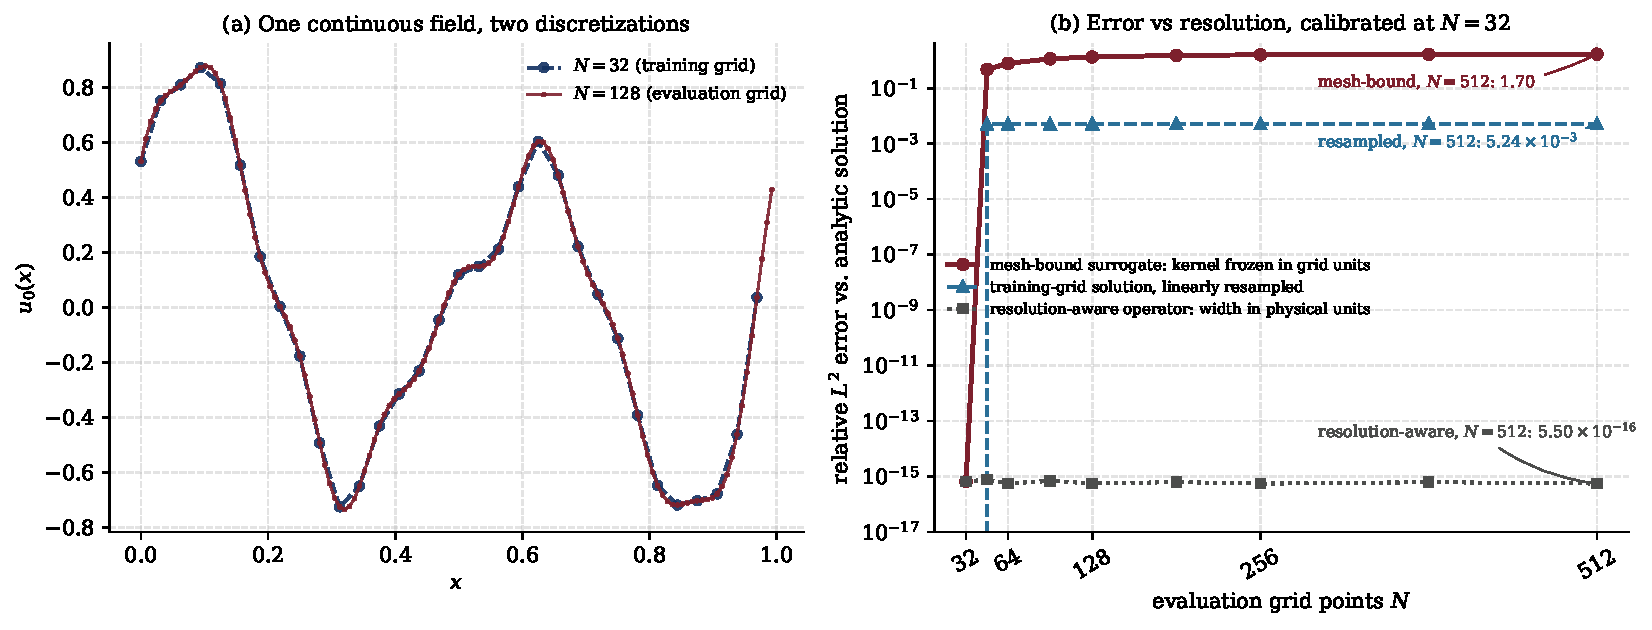
\includegraphics[width=0.92\textwidth]{fig_super_resolution.pdf}
\caption{\textbf{Resolution transfer versus mesh-bound degradation.} (a) The same continuous field from the band-limited input family of Appendix~\ref{app:b}, sampled on a coarse ($N=32$) and a fine ($N=128$) grid of $\mathbb{T}=[0,1)$. (b) Relative $L^2$ error against the analytic heat solution at $T=1$, averaged over 80 inputs, as the \emph{evaluation} grid is refined from $N=32$ to $N=512$ with all operators calibrated at $N=32$. \textbf{No curve, line or marker stands for a trained network:} the one-layer FNO of Appendix~\ref{app:b} is quoted in Section~\ref{sec:appb-result}
and not plotted here, because every curve this plate draws is computed from a solved model;
the trained run's own numbers are quoted in Appendix~\ref{app:b}, whose log and archive are
held with the book. The three curves are computed from discretization error alone and are not trained networks: a mesh-bound smoothing operator whose kernel width is frozen in \emph{grid} units gradually stops smoothing as $N$ grows, reaching $1.70$ at $N=512$; the same operator with its width stated in \emph{physical} units tracks the analytic solution to between $5.48\times10^{-16}$ and
$7.63\times10^{-16}$ on every grid; and solving on the training grid then resampling
linearly plateaus at the interpolation error of the coarse solve, $5.24\times10^{-3}$. \textbf{Caveat, stated once and not to be forgotten:} the test inputs contain only eight Fourier modes and are therefore already fully resolved on the coarse training grid, so the fine-grid evaluation resamples the \emph{same} continuous functions. What the three curves show is what refinement does to a discretization; resolution
transfer of a learned operator is the claim of the quoted experiment of
Appendix~\ref{app:b}, and nothing drawn here establishes it, let alone recovery of
unresolved high-frequency detail. The governing equation is the linear heat equation, whose solution operator is the explicit multiplier $e^{-\alpha(2\pi k)^2 T}$; the network is a teaching example, not evidence that FNOs outperform classical solvers.}
\label{fig:super_resolution}
\end{figure}

Figure~\ref{fig:super_resolution} puts the mechanism and its computed consequences side by
side. Panel (a) shows one continuous field on two discretizations, which is the
operation an invariant model must survive. In panel (b) the mesh-bound curve
degrades exactly as \eqref{eq:ch06-receptive} predicts, the resolution-aware
curve stays at the level of roundoff on every grid, and resampling a
training-grid solution flattens out at the interpolation error of the coarse
solve --- the honest price of the ``interpolate, then run'' workaround. The trained model of Appendix~\ref{app:b} is not in this panel: its reported errors,
$0.0141$ at $N=64$ and the same at $N=256$, are printed by the run re-executed for this book and
archived at \texttt{artifacts/appendix\_b\_run.txt}, and are quoted in
Section~\ref{sec:appb-result} rather than plotted.

What that pair of numbers establishes must be read carefully, and the reading is
less flattering than the usual headline. The inputs carry eight Fourier modes
and are fully resolved on the sixty-four-point grid, so no unresolved detail is
being recovered --- the experiment demonstrates
\emph{resolution transfer}\index{resolution transfer|textbf}, not super-resolution
in the sense of imaging. Moreover the network has a single Fourier layer, so
Proposition~\ref{prop:ch06-zeroshot} applies to its spectral branch with almost
nothing left over. The lift is linear and therefore preserves the band limit;
the twelve retained bins of the real transform cover wavenumbers $0$ through
$11$, so $k_{\max}=11$ sits above the input bandwidth $8$ and far below
$N/2=32$, leaving the Nyquist-type hypothesis of the proposition room to spare;
and the only band-limit-breaking step, the pointwise activation, is not
followed by any further transform. The two discrete norms behind the
identical $0.0141$ are Riemann sums of the same real-analytic error field on
two grids, so their difference is an exponentially small quadrature error, far
below the four decimals that were printed. Both reported numbers are
therefore one number: a model error of order $1.4\%$, printed twice. Both come from one execution, re-run for this book; the archive holds an exemplar
pair rather than the test-set metric, so the printed averages remain the record.
Nothing in the figure shows accuracy at resolutions the data never contained,
and nothing in it shows an advantage over classical solvers for a linear problem
that a single Fourier multiplier solves exactly. That a model \emph{can be
evaluated} on any compatible grid is an architectural property; that it is
\emph{accurate} there is an empirical claim, and it must be re-verified per
problem. The FNO benchmark literature reports models trained on
$64\times64\times20$ space-time data evaluated at $256\times256\times80$
\cite{li2021fourier}, and such reports are observations about the benchmarks
they were run on. The nonlinear, multi-scale problems that motivate operator
learning in the first place are exactly the ones where retained-mode truncation
and sharp moving fronts interact, and where accuracy at a new resolution has to
be demonstrated rather than inferred --- in heterogeneous multiphase flow, the
standard spectral layer resolves fronts less well than an architecture
augmented for fine scales \cite{wen2022ufno}.

\section{Continuum Rates and the Separation of Error Sources}
\label{sec:ch06-rates}

The gap between the exact identity \eqref{eq:ch06-zeroshot} and real multi-layer
networks on rough data is a discretization
error\index{discretization error!algebraic rate} of a particular kind: it sits
between the continuum definition of an FNO and its grid-based realization, with
the parameters held fixed, and is therefore distinct from approximation error
and from estimation error. The estimate this book uses for that gap is the
following.
Write $\Psi_{\text{FNO}}$ for the
continuum network determined by a fixed $\theta$ and $\Psi_{\text{FNO}}^N$ for
its implementation on the $N^d$ grid, and let $v_t$ and $v_t^N$ denote the
corresponding states after $t$ layers. Under the assumptions that the
activations possess bounded continuous derivatives up to order $s$, that the
input set $\mathcal{A}$ is contained in $H^s(\mathbb{T}^d)$ with $s>d/2$, that
the retained modes satisfy $k_{\max}<N/2$, and that the layer parameters are
bounded in the natural norms, the grid error obeys, for every compact
$\mathcal{A}_c \subset \mathcal{A}$,
\begin{equation}
  \label{eq:ch06-rate}
  \sup_{a \in \mathcal{A}_c} \frac{1}{N^{d/2}} \big\| v_t(a) - v_t^N(a) \big\|_{\ell^2(\{x_n\})} \;\le\; C\, N^{-s},
\end{equation}
with $C$ depending on the activation bounds, the parameter bounds, $d$, $s$, the
layer index $t$ and $\mathcal{A}_c$, and the $\ell^2$ norm taken over the $N^d$
nodes of the grid. The same rate holds at the continuum level, with
$\|\Psi_{\text{FNO}}(a)-\Psi_{\text{FNO}}^N(a)\|_{L^2(\mathbb{T}^d)}$ in place of
the grid norm, once the discrete states are replaced by their trigonometric
interpolant. The decay is algebraic, and its
exponent is the Sobolev regularity of the input, inherited by the states it
produces --- the very currency
\chapref{ch:part1-function-spaces-duality-and-sobolev-regula} introduced.

""
elementary, but bounding an entire network requires controlling
$\|v_t\|_{H^s}$ through compositions of nonlinear maps, and that regularity
propagation is where the whole difficulty of \eqref{eq:ch06-rate} sits.
The smoothness requirement is not decorative either, since the exponent is
capped by the least regular object in the pipeline: the rectified linear unit
(ReLU) has regularity only just below $H^{3/2}$ --- its derivative is a step
function --- so with ReLU the decay in \eqref{eq:ch06-rate} saturates once the
input is smoother than that, the ceiling being a property of the activation
rather than of the data, whereas smooth activations such as the Gaussian error
linear unit (GeLU) leave the input regularity to set the rate
\index{ReLU activation!rate saturation}\index{GeLU activation}.
Appending \emph{non-periodic} positional coordinates to a smooth input --- a
standard trick in practical FNO implementations --- introduces a jump across the
boundary of $[0,1]^d$, hence regularity $H^{1/2-\epsilon}$ for every
$\epsilon>0$ and no better, so the exponent available in \eqref{eq:ch06-rate}
falls just short of $1/2$ however smooth the physical channels are.
And the constant grows with the layer index, so the smallness of
\eqref{eq:ch06-rate} is a statement about bounded parameters, not about
well-trained ones. The bound constrains a fixed $\theta$; it says nothing
about whether the $\theta$ obtained by training on grid $N$ coincides with the
one a doubled grid would have produced.

The bookkeeping this suggests is worth writing down once. Let
$\mathcal{E}(n,k_{\max},N)$ denote the error with which a surrogate, trained on
$n$ paired samples stored on the $N$-point grid with $k_{\max}$ retained modes,
reproduces the operator it was trained toward, measured on that same grid. Up
to a multiplicative constant, that error splits as
\begin{equation}
  \label{eq:ch06-decomp}
  \mathcal{E}(n,k_{\max},N)
  \;\lesssim\;
  \underbrace{\mathcal{E}_{\mathrm{stat}}(n)}_{\text{statistical}}
  \;+\;
  \underbrace{\mathcal{E}_{\mathrm{trunc}}(k_{\max})}_{\text{truncation}}
  \;+\;
  \underbrace{\mathcal{E}_{\mathrm{disc}}(N)}_{\text{discretization}},
\end{equation}
a separation made explicit, and rigorous with matching upper and lower bounds for
a discrete-Fourier-transform least-squares estimator of the linear FNO layer, by
Subedi and Tewari \cite{subedi2024controlling}\index{error decomposition!statistical, truncation, and discretization|textbf}.
The truncation term is the spectral truncation of
Theorem~\ref{thm:fno_convergence}, decaying like $k_{\max}^{-\alpha}$ where
$\alpha$ is the smoothing order of that theorem; the discretization term is
\eqref{eq:ch06-rate}; and the statistical term is the generalization error of the
fit, whose sharp form for the operator classes this book learns --- a matching
lower bound, and an estimate whose statistical part does not move with $N$ ---
\chapref{ch:part1-open-theoretical-problems-and-mathematical} lists as open.
Equation \eqref{eq:ch06-decomp} has an immediate practical reading, and it is
the one usually inverted: refining the grid buys nothing once $N^{-s}$ has
dropped below the statistical and truncation floors, while a generous dataset
and a generous $k_{\max}$ can expose a grid error that coarse experiments were
masking. Read in the other direction, the decomposition licenses cheapness ---
if the discretization term dominates early in training, there is no reason to
compute to higher accuracy than the model error --- and that is the logic of
\emph{adaptive subsampling}\index{adaptive subsampling}: train first on a coarse
grid and double the resolution when the validation error plateaus rather than
continuing to improve. Of the three terms of \eqref{eq:ch06-decomp} only
$\mathcal{E}_{\mathrm{disc}}(N)$ responds to refinement, so a loss that stops
falling at fixed $N$ may be resting on the discretization floor rather than on a
model that has stopped learning, and one refinement step is the cheapest
diagnostic that distinguishes the two.

\takeaway{Invariance Is an Architectural Property; Accuracy Is an Empirical One}{%
A neural operator's parameters are indexed by functions rather than by positions
in an array, so one $\theta$ defines a continuum map and a consistent discrete
realization
linked by \eqref{eq:limit_commute}. Exact transfer across grids holds only under
the band-limitedness and Nyquist-type hypothesis $N>2k_{\max}$ of
Proposition~\ref{prop:ch06-zeroshot}; in general the discrete-to-continuum gap
decays algebraically, like $N^{-s}$ with $s$ the Sobolev regularity of the input,
as in
\eqref{eq:ch06-rate}. The reported equality of errors at the $64$- and
$256$-point grids, quoted from Appendix~\ref{app:b} and not plotted in
Figure~\ref{fig:super_resolution}, shows resolution transfer on inputs the coarse grid already
resolved --- not recovery of lost detail, and not superiority over classical
solvers.}

Two questions remain unanswered by \eqref{eq:ch06-decomp}, and both shape the
next chapter. First, the accounting presumes labeled solution data on every grid
it prices: it says how to bill an experiment, not how to learn when labels are
scarce. Second, the errors in \eqref{eq:ch06-rate} and
\eqref{eq:ch06-decomp} are measured in $L^2$-type norms, which constrain the
size of a mistake but not its oscillation --- a surrogate can be accurate in the
mean while its derivatives, and with them its fluxes and its fronts, are wrong.
The remedy in both directions is to put the differential equation into the
objective. The spectral
differentiation that a residual-based loss needs is the same
trigonometric-interpolation machinery that justified \eqref{eq:ch06-zeroshot},
now used to differentiate rather than to resample; and an objective weighted in
$H^1$ or $H^2$ prices exactly the regularity that sets the exponent in
\eqref{eq:ch06-rate}. \chapref{ch:part1-physics-informed-operators-and-sobolev-reg}
develops that move through the physics-informed neural operator
(PINO) \cite{li2021physics} and Sobolev-regularized losses, showing how the
residual term and the mesh-consistent normalization of the objective work
together, and turning the mesh-transfer question raised here into a
training-time constraint.
